\chapter{Basic Machine Learning}\label{ch:knnkm}

As an example of Machine Learning algorithms, in this chapter we discuss the Classification algorithm of $k$-Nearest Neighbours and the Clustering algorithm of K-Means. As shown in section \ref{sec:aai} there are many more machine learning methods, the two presented here provide a good and generic introduction into the field of machine learning.

\section{Classification: $k$-nearest neighbours}\label{sec:knn}

Classification is the generic process of trying to categorise something. It encompasses the process in which ideas or objects are recognized, differentiated, and understood (put in some class). In general, classification is the problem of trying to identify to which set of categories (also called sub-populations or \emph{classes}) a new observation belongs. Observations can relate to physical objects (e.g., people, animals, books, etc.) or more abstract concepts (like events, ideas, etc.). The categorisation is done based on a given training set of data containing observations (instances) whose category membership is known. An example is ``spam'' filtering, where incoming (before unseen) emails are categorised as either ``spam'' or ``ham'' (not-spam)\footnote{SPAM\copyright\ was a type of canned cooked meat popularized after the second world war, which was not quite ham. The use of the word for unsolicited (electronic) advertisement was derived from the Monty Python sketch, in which the word was increasingly inserted into the conversation \cite{spam}.} given a body of emails of which it is known (or has been indicated) whether they are ``spam'' or ``ham''.

The availability of a training set of which the class membership is known, makes classification a \textbf{supervised} machine learning technique. An algorithm that implements classification is known as a \textbf{classifier}. It can be seen as a function that maps input data to a category.

A classification algorithm examines the individual observations (\textit{instances)} and analyses of each of them a set of quantifiable properties, known as \textit{explanatory variables} or \textit{features}. These can be, for example, $age$, $length$, $weight$, etc. of a human being (to be classified as `adult' or `child'), or the relative frequency of the occurrences of ``spammy words'' in an email. A combination of such quantifiable properties is called a \textit{feature vector}.

A feature vector is a $n$-dimensional vector (it contains $n$ attributes) of numerical features that represents some object\footnote{When a variable $x$ is in fact a vector, we will indicate that with an overset arrow: $\vec{x}$ for clarity. The different attributes of $\vec{x}$, we typically number from $1$ to $n$: $\vec{x}=(x_1,\ldots,x_n)$. A random attribute of $\vec{x}$ is indicated as $x_i$.}. For instance, our representation of a human being, mentioned above, by $age$, $length$, and $weight$ has 3-dimensional feature vector. More concretely, the feature vector $(56, 185, 81)$ is then the representation of `Barack Obama'. When representing images, the feature values might correspond to the pixels of an image, while representing texts the features might be the frequencies of occurrence of textual terms.

The \textit{vector space} can then be understood as space that can contain all the possible values in the feature vectors, and represents a complete picture of the domain. Each feature of the feature vectors relate to a single dimension of the vector space, in much the same way as the x, y and z position (feature) of a point relates to a position on the x-, y- and z-axis of a graph. A feature vector with 20 attributes thus relates to a 20-dimension vector space (which can be difficult to grasp, or graph).

\textit{Classes} or \textit{categories} can then be understood as a particular partition (section) of the vector space, where all instances that fall into that partition are considered to be of the same `type'. Note that the differentiation between classes can be made on a single feature (e.g., everyone below the age of 18 is considered `child', everyone above is an `adult'), or a combination of features (e.g., specific combinations of length and weight are considered healthy, others are considered unhealthy).

\subsection{Intuitions}
There are multiple ways to perform classification. One could use Bayesian (probability) based calculations or statistical (Gaussian) models to predict the probabilities that a particular observation belongs to a particular class. These models can be extremely powerful, but are rather cumbersome with (complex) mathematics. Instead, we introduce the \textit{$k$-Nearest Neighbours algorithm}, which performs in a very similar way as that we humans would, which makes it much easier to understand.

Consider the classification problem presented below in Figure \ref{fig:intuition}. This is a typical classification problem; we have a training set of labelled data (the red circles and the blue triangles), and have been given the task to determine whether a new observation (the white box) is either a red circle or a blue triangle.

When given the task of trying to determine the class of the box in Figure \ref{fig:intuition}, humans do not calculate the priors of it belonging to `blue' or `red', nor do humans use statistics to predict the probability of it being `red' (or `blue'). Instead, humans will eyeball the image, and (correctly) determine that the box will \textit{probably} be a `red circle', merely on the fact that it is \textit{much closer} to the red examples, than to the blue examples. This intuition of classification based on closeness is what drives the $k$-Nearest Neighbour algorithm.

\begin{figure}[h!]
\begin{center}
\begin{tikzpicture}
\node[anchor=south west, inner sep=0] at (0, 0) {\includegraphics[width=0.75\textwidth]{classification}};
% \draw[step=1cm,gray,very thin] (0, 0) grid (9, 7);
\draw[white, fill=white] (5, 4) rectangle (5.5, 3.5);
\node at (6, 4.25) {?};
\end{tikzpicture}
\end{center}
\caption{Classification problem: to which class does the box belong?}\label{fig:intuition}
\end{figure}

While with a more complex vector space (our example uses only two features, since it is easier to plot) a human could not eyeball it any more, as long as can come up with some measure of `closeness', we could still apply the same principles to determine classes of observations in, say, a 20-dimensional feature space.

In essence, by looking at the closest neighbour (of which we know the class), we are partitioning the vector space into parts where the boundaries between two points is determined by the fact that every point on the boundary is an equal distance to either point. This type of partitioning is called \textit{Voronoi tesselation}. Figure \ref{fig:voronoi} below shows an example of such a Voronoi tesselation (right) of the vector space shown (left). By looking at the position of the box, it can now be determined that in the problem presented in Figure \ref{fig:voronoi}, the box is closest to a blue triangle (it is within the region of a triangle) and is therefore probably a triangle.

\begin{figure}[h!]
\begin{center}
\begin{tikzpicture}
\node[anchor=south west, inner sep=0] at (7, 0) {\includegraphics[width=0.55\textwidth, trim={1.75cm 1cm 1.5cm 1cm},clip]{classification2-vor}};
\node[anchor=south west, inner sep=0] at (0, 0) {\includegraphics[width=0.55\textwidth, trim={1.75cm 1cm 1.5cm 1cm},clip]{classification2}};
\node at (5.1, 3.7) {\small ?};
\end{tikzpicture}
\end{center}
\caption{Feature space (left) and Voronoi tesselation (right).}\label{fig:voronoi}
\end{figure}

The combinations of all regions of the triangles and all the regions of the circles defines the transition of when a new observation is classified as either a triangle or as a circle. This is the boundary between the set of regions of either example, and is called the \textit{classification boundary}. Figure \ref{fig:boundary} below shows the classification boundary for the given example. Observations to the left of the classification boundary are classified as triangle, those to the right of it are classified as circles.

\begin{figure}[h!]
\begin{center}
\begin{tikzpicture}
\node[anchor=south west, inner sep=0] at (0, 0) {\includegraphics[width=0.8\textwidth]{classification2-vor}};
% \draw[step=0.1cm,gray!20,very thin] (0, 0) grid (10, 7);
% \draw[step=1cm,gray,very thin] (0, 0) grid (10, 7);
\draw[ultra thick, red] (3.3, 7) -- (4.2, 5.8) -- (5.9, 5.3) -- (6.3, 5.7) -- (7.3, 4.6) -- (7.1, 4.2) -- (7.2, 3.9) -- (6.8, 3.1) -- (6.1, 2.9) -- (5.8, 2.8) -- (5.3, 2.8) -- (5.2, 1.9) -- (4.4, 0.8);
\end{tikzpicture}
\end{center}
\caption{Classification boundary for $k$-NN with $k=1$.}\label{fig:boundary}
\end{figure}

Note that the classification boundary is not linear, and reflects well the different classes, which is rather impressive for such a simple algorithm. However, this method is not without its problems, as we see in the following Section.

\subsection{Outliers}
The classification problem presented above was rather straight-cut. While the classification boundary has a rather complex shape, the training set is still very neat (all triangles are on one side, the circles on the other). In reality, it often happens that training samples are much more scattered throughout each other. In some extreme cases, we speak of outliers (see Figure \ref{fig:outlier} below). The single red circle on the left side of the feature space is an odd duck, and could be the result of some error (perhaps noise during measurement or a typo in the data), but it could also be that our classification examples are not as clear as we have seen above.

\begin{figure}[h!]
\begin{center}
\begin{tikzpicture}
\node[anchor=south west, inner sep=0] at (0, 0) {\includegraphics[width=0.8\textwidth]{classification2-vor}};
% \draw[step=0.1cm,gray!20,very thin] (0, 0) grid (10, 7);
% \draw[step=1cm,gray,very thin] (0, 0) grid (10, 7);
\draw[white, fill=white] (3.1, 3.9) rectangle (3.5, 4.1);
\draw[black, fill=red, thick] (3.35, 4) circle (0.05cm);
\draw[ultra thick, red] (3.3, 7) -- (4.2, 5.8) -- (5.9, 5.3) -- (6.3, 5.7) -- (7.3, 4.6) -- (7.1, 4.2) -- (7.2, 3.9) -- (6.8, 3.1) -- (6.1, 2.9) -- (5.8, 2.8) -- (5.3, 2.8) -- (5.2, 1.9) -- (4.4, 0.8);
\draw[ultra thick, orange] (1.4, 5.5) -- (4.6, 4) -- (4.6, 3.4) -- (1.4, 3.4);
\end{tikzpicture}
\end{center}
\caption{An outlier and the effect on the classification boundary (orange).}\label{fig:outlier}
\end{figure}

Suddenly, the classification boundary is even more complex, and non-continuous. There now is some region in which instances are classified as triangles (between the orange and red lines) and everything else is classified as circles. Again, this is a simplified view to highlight a problem, more outliers will increase the complexity of the classification boundary even further. 

If the single circle on the left of the training set is indeed an error, this shows that errors can have strong effects on the outcome of the classifier. A single error radically changes the shape of the classification boundary, and this is unwanted; the boundary exactly follows the training data. 

Until now, we have only looked at a single neighbour of an instance. If we take more neighbours into consideration (e.g., the closest 3 or the closest 5) and use those to determine the class of a new observation, the classifier becomes much more stable. In this sense, we take the closest $k$\footnote{Hence the name of the algorithm.} training samples and derive a class from them (e.g., by taking a mean, or a majority vote). In our example above (see Figure \ref{fig:outlier}), the number of triangles on the left side of the image will outweigh the single circle, thus removing its destructive effect on the classification boundary.

\begin{aside}[Overfitting vs. underfitting]\label{as:overfit}\mbox{}\\
The problem described above, when a learned boundary, or other property that is derived from the data, exactly models the training data is called \textit{overfitting}. In essence, you have made a single perfect classifier for one set of data: the classifier will work flawlessly on the training data, but can perform significantly worse on other (new) data.

When using machine learning, it has to be taken into account that one is typically working with noisy data. That is, the samples that you have to train your algorithm are \textit{not} an exact representation of the problem/solution. There could be parts missing, or the data available could be distorted by noise, etc. Whatever the problem might be, it is never a wise decision to exactly model the training data available, since your algorithm looses all possibilities of generalising to other (similar, but slightly different) instances that have not yet been seen.

\begin{center}
\includegraphics[width=0.5\textwidth]{Overfitting}\\
\begin{minipage}{0.6\textwidth}
The green line shows an overfitted model, exactly following the training data. The black line shows a regularised model.
\end{minipage}
\end{center}
\unfootnote{Image by Wikipedia.}
The opposite of overfitting is \textit{underfitting}, when you design your algorithm too loosely. In that case, the classifier will not be precise enough with respect to the instances presented. Training machine learning algorithm is often trying to find a balance between the two.
\end{aside}

\subsection{The $k$-NN algorithm}
Now we understand the intuition behind distance based classification, we can introduce the $k$-Nearest Neighbours ($k$-NN) algorithm. The $k$-NN algorithm is given below:
\begin{algorithm}[$k$-Nearest Neighbours]\label{al:knn}\mbox{}\\
Given:
\begin{itemize}
\item Training set $X$ of examples $(\vec{x_i}, y_i)$ where
\begin{itemize}
\item $\vec{x_i}$ is feature vector of example $i$; and
\item $y_i$ is class label of example $i$.
\end{itemize}
\item Feature vector $\vec{x}$ of test point that we want to classify.
\end{itemize}
Do:
\begin{enumerate}
\item Compute distance $D(\vec{x}, \vec{x_i})$;
\item Select $k$ closest instances $\vec{x_{j_1}},\ldots,\vec{x_{j_k}}$ with class labels $y_{j_1},\ldots,y_{j_k}$;
\item Output class $y^*$, which is most frequent in $y_{j_1},\ldots,y_{j_k}$.
\end{enumerate}
\end{algorithm}
The $k$-NN algorithm is simple to understand. We take our new observation $\vec{x}$ and compare that to all available training examples, by computing the distance $D(\vec{x}, \vec{x_i})$ between the two. Next, we select the $k$ closest training samples to $\vec{x}$ and collect their labels $y_{j_1},\ldots,y_{j_k}$. We can then determine the answer by selecting the label $y^*$ by looking which label occurs most often.

There are multiple ways to calculate distances between vectors, but for now we use the Euclidean distance (straight-line distance between two points\footnote{The calculation of the Euclidean distance is a straight-forward application of the law of Pythagoras: the distance $d$ between points $(a_1,\ldots,a_n)$ and $(b_1,\ldots,b_n)$ is $d^2=(a_1-b_1)^2+\ldots+(a_n-b_n)^2$.}).

\begin{aside}[Distance measures]\label{as:distance}\mbox{}\\
So far we have only considered the most straightforward distance measure to determine the distance between points (in both K-Means and in $k$-Nearest Neighbours). This measure, Euclidean distance, is the straight-line distance between two points in space, like "as the crow flies" in geometric distances (``vogelvluchtafstand''). It is an intuitive and much used distance measure, but it has some drawbacks.

A drawback of Euclidean distance is that it evaluates all the dimensions of the points equally important. That is, given a 2-dimensional problem (where points have an x-value and an y-value), Euclidean distances considers a step on the x-axis as important as a step on the y-axis. That is, $(2,1) \leadsto (2,2)$ is as far apart as $(2,1) \leadsto (3,1)$. This can produce big differences when the scale of each of the dimensions is different. For instance, when $x$ represents $age$ and $y$ represents $gross income$, the influence of $y$ on the distance between two points is much larger than that of $x$ (as $y$, for typical people, is measured in thousands (of euros), while age is measured in single years.

Other, numerical, distance measures available are:
\begin{itemize}
\item\textbf{Manhattan Distance}: the distance between two points calculated by strict horizontal and/or vertical paths (that is, along the grid lines), as opposed to the diagonal ("as the crow flies") Euclidean distance.
\begin{center}
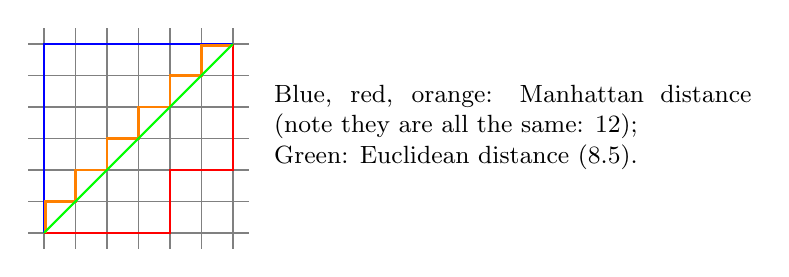
\begin{tikzpicture}[scale=0.4]
\begin{scope}
  \draw[step=1cm,gray] (-0.5, -0.5) grid (6.5, 6.5);
  \clip (0, 0) rectangle (6, 6);
\end{scope}
\draw[blue, thick] (0, 0) -- (0, 6) -- (6, 6);
\draw[red, thick] (0, 0) -- (4, 0) -- (4, 2) -- (6, 2) -- (6, 6);
\draw[orange, thick] (0.05, 0) -- (0.05, 1) -- (1, 1) -- (1, 2) -- (2, 2) -- (2, 3) -- (3, 3) -- (3, 4) -- (4, 4) -- (4, 5) -- (5, 5) -- (5, 5.95) -- (6, 5.95);
\draw[green, thick] (0,0) -- (6, 6);
\node[anchor=north west] at (7, 5) {\begin{minipage}{0.5\textwidth}\small Blue, red, orange: Manhattan distance (note they are all the same: 12);\\ Green: Euclidean distance (8.5).\end{minipage}};
\end{tikzpicture}
\end{center}
\item\textbf{Minkowski Distance}: a generic measure of distance, generalised from the Euclidean and Manhattan distance described above. Minkowski distance is calculated by: $\sqrt[p]{\sum^{n}_{i=1}|x_i-y_i|^p}$\\
When $p$ is $1$, this equates to the Manhattan distance, when $p$ is $2$ one gets the Euclidean distance. With $p$ reaching $\infty$, one obtains the Chebyshev distance.
\begin{center}
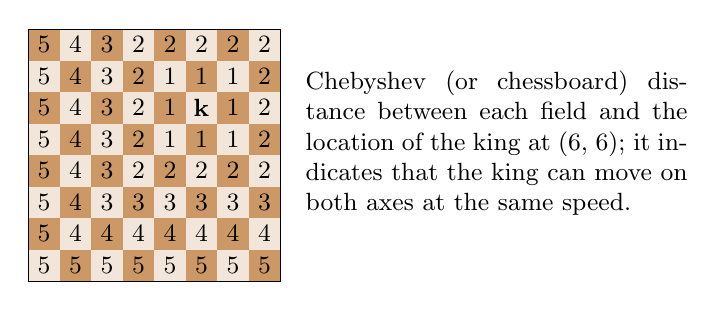
\begin{tikzpicture}[scale=0.4]
\foreach \x in {0,...,7} \foreach \y in {0,...,7}
  {
    \pgfmathparse{mod(\x+\y,2) ? "brown!80" : "brown!20"}
    \edef\colour{\pgfmathresult}
    \path[fill=\colour] (\x,\y) rectangle ++ (1,1);
    \pgfmathparse{max(abs(\x-5), abs(\y-5))}
    \edef\distance{\pgfmathresult}   
    \node at (\x+0.5, \y+0.5) 
        {\small\pgfmathprintnumber{\distance}};
  }
\draw (0,0)--(0,8)--(8,8)--(8,0)--cycle;
\path[fill=brown!20] (5,5) rectangle (6,6);
\node at (5.5, 5.5) {\small\textbf{k}};
\node[anchor=north west] at (8.5, 7) {\begin{minipage}{0.4\textwidth}\small Chebyshev (or chessboard) distance between each field and the location of the king at (6, 6); it indicates that the king can move on both axes at the same speed.\end{minipage}};
\end{tikzpicture}
\end{center}
\item\textbf{Chebyshev Distance}: this measure defines the distance between two vectors as the greatest of their differences along any coordinate dimension. It is best visualised by the moves of a king on a chessboard (see above).
\end{itemize}

Another disadvantage is that Euclidean distance only works for numeric attributes on an interval or ratio scale. For categorical scales (e.g., $gender$ or $hair\ colour$) it is impossible to calculate a Euclidean distance. Instead, one can use the \textbf{Hamming Distance}, which counts the number of substitutions (changes) that need to be made to get from one sample to another. That is to say, it counts the number of attributes that are different between two given points.
\end{aside}

The selection of the resulting class label from the set of labels $y_{j_1},\ldots,y_{j_k}$ can be understood as a majority vote. Each $y_j$ in the set counts as a ballot (`stembiljet') in the vote, and the class that is selected the most is considered the winner.

\subsection{Problems with $k$-NN}
While $k$-NN is intuitively simple it performs quite well for such a simple algorithm. However, there are some inherent problems with $k$-NN, that we address here.
\subsubsection{How to choose K?}
The biggest question when applying the $k$-NN algorithm, is how to determine the best $k$; that is, how many neighbours should you look at to get the best (stable) result in your classification.

The choice of the value of $k$ has a strong effect on the performance of $k$-NN. If the $k$ is chosen too large, everything will be classified as the class that is most common in the data (that is, the one that has the most ballots in the vote). When $k$ approaches the size of your training set, the closeness to samples of a particular class have no longer an influence on the classification, but the amount of samples that are available (of each class) in the data set start to overrule the vote.

If the value of $k$ is chosen too low, as we have seen before, the classifier becomes less stable, and is much more receptive to the influence of outliers. This leads to an unstable classification boundary. The value of $k$ has a large impact on the smoothness of the classification boundary.

\begin{figure}[h!]
\begin{center}
\begin{tikzpicture}
\node[anchor=south west, inner sep=0] at (0, 0) {\includegraphics[width=0.8\textwidth, trim={3cm 2cm 3cm, 2cm},clip]{kNN}};
\node at (5.3, 4.5) {?};
\node at (6.5, 3) {$k=3$};
\node at (5.5, 2.4) {$k=4$};
\node at (5.5, 1.7) {$k=5$};
\node at (5.5, 0) {$k=n$};
\end{tikzpicture}
\end{center}
\caption{The influence of the value of $k$.}\label{fig:kNN}
\end{figure}

See Figure \ref{fig:kNN}: 
\begin{itemize}
\item $k=1$ will classify the green circle as a red triangle;
\item $k=3$ will still classify it as a red triangle;
\item $k=4$ leads to a tie (see next Section);
\item $k=5$ changes classification to a blue square;
\item $k=n$ keeps classification as blue square (there are more square examples than triangle examples in the training data).
\end{itemize}

To select the proper $k$, we have to use a technique often applied in machine learning. We set aside a portion of the training data (i.e., those randomly selected samples of which we know the class are removed from the set of samples given to the algorithm); this set is called the \textit{validation set}. Next we run the algorithm with different sizes of $k$ and test on this validation set which number of $k$ performs the best on classifying the validation samples. Since we know the class of each of the samples in the validation set, we can calculate a classification error for each $k$ based on the number of correct/incorrect classifications made by the algorithm. We can now determine the best $k$, we select the $k$ that gives the best generic performance.

\subsubsection{Resolving ties}
It can occur that the classification vote ends in a tie (see the example in Figure \ref{fig:kNN} above). In those rare cases when there are an equal amount of positive and negative votes there are a number things to do:
\begin{itemize}
\item \textbf{Use an odd $k$}: when dealing with binary classification, using an odd number of neighbours in the vote makes it impossible to have as much positive as negative votes. However, when dealing with a multi-class classification problem (where there are more than two classes), this solves nothing, however, as ties can still occur.
\item \textbf{Breaking ties}: other possibilities of solving ties are:
\begin{itemize}
\item At random: choose a class at random (by flipping a coin). The rational is that it does not matter, as the observation is obviously on the border between the two classes.
\item Use the \textit{prior}; that is, choose the class that is most often occurring in the training set. The rational is that, since the prior is more common (more occurring), the probability that you guess right by selecting that class is higher.
\item \textbf{Nearest}: use a lower $k$ (e.g. $k=1$, since that will never result in a tie) to select the class.
\end{itemize}
\end{itemize}

\subsubsection{Why is $k$-NN slow?}
While $k$-NN performs well for its complexity, it not a very forgiving algorithm. With larger training sets, the performance (time/memory it takes to calculate an answer) becomes increasingly worse.

The main problem of $k$-NN is the fact that, since the computer has no representation of distance, dimensions or closeness. In order to assess a new observation given a training set of data, it has to compute the distance of the observation to each of the available training samples. And with large amounts of training data available (which tends to increase the robustness of your classifier), the classifier will perform slower and slower. In the same way, each additional dimension in the features of samples increases the amount of calculations needed to compute the nearest $k$ elements (which is why it often helps to reduce dimensions, see Section \ref{sec:aai}, \emph{before} using $k$-NN).

Consider the Figure \ref{fig:slow} below.

\begin{figure}[h!]
\begin{minipage}{0.45\textwidth}
What you see:\\
\includegraphics[width=\textwidth, trim={2.5cm 1.5cm 2.5cm 1.5cm}, clip]{kNN-slow}
\end{minipage}\hfill
\begin{minipage}{0.55\textwidth}
What the computer sees:
\begin{framed}
\begin{lstlisting}
data = np.array([
 (1, 9), (2, 3), (4, 1), (3,7),
 (5, 4), (6, 8), (7, 2), (8, 8),
 (7, 9), (9, 6)
])
testPoint = (7, 4)
\end{lstlisting}
\end{framed}
\end{minipage}
\caption{Comparison: find the nearest neighbour to the red cross.}\label{fig:slow}
\end{figure}

To the computer, the training data is just an array of feature vectors, which each have to be compared to \pythoninline{testPoint} to calculate the distance. For a training set of $n$ samples, with $d$ features, this takes $n*d$ comparisons for every point you try to classify.

The easiest fix for this problem, as mentioned above, is the removal of (a number of) dimensions. This can be done in a simplistic way, by throwing away attributes that are not important to the classification process; e.g. in our earlier example, where we represented humans as a vector of $(age, length, weight)$, and try to classify them as `child' or `adult', we can remove the $length$ and $weight$ attributes. For more complex dimensional reduction, one could use more complex (mathematical) techniques such as Principle Component Analysis, which tries to find the most discriminative dimensions (which could be combinations of some of the dimensions in the feature space).

Another fix would be by reducing the number of training examples. The idea here is identify a small number of individuals $m \ll n$ of potential neighbours, and use only those to classify new observations. In essence, you are trying to find \textit{prototypical examples} of the classes, and use those to do the classification. This idea is exploited in the K-D Trees algorithm (which can be thought of as a combination of $k$-NN and decision trees; exploiting the best of both techniques).


\section{Clustering: K-Means}\label{sec:kmeans}
Clustering is the problem of trying to determine whether there is any underlying structure in the data that is available. For instance, if you have data about a number of individuals, can those individuals be grouped in some way(s) such that members of each group seemingly belong together, yet also not appear to be belong to some other group. 

That is, clustering tries to come up with groups (called \textit{clusters}) such that the intra-cluster distance is minimised, yet the inter-cluster distance is maximised. The intra-cluster distance is a measure of the similarity of objects within a group (how much are they similar to each other); the inter-cluster distance is the difference (from the group as a whole) to other groups that have been identified.

Clustering is typically an \textbf{unsupervised} task as it does not try to predict anything specific. It tries to find sub-populations in the data, but it can be difficult to figure out how many of those there are and what their size is? Moreover, are the clusters based on common properties and are the clusters cohesive or can they be split further?

This latter aspect of clustering, whether elements in a cluster have common properties, differentiates between two forms of clustering: monothetic and polythetic clustering. \textit{Monothetic clustering} groups members on a single common property, for instance, all elements have an age between 20 and 35 years, or each has a particular answer to a particular question of an inquiry. \textit{Polythetic clustering}, on the other hand, groups elements based on similarity, where the similarity is not driven by a single common property. Based on all attributes of the elements, the distance between the elements alone defines their membership to the different groups (that is, all attributes are considered to determine group membership).

Another important difference between clustering algorithms is whether the clusters can have an overlap. \textit{Hard clustering} are those algorithms that assign a unique group to each element, meaning that elements belong to a cluster or it does not belong to that cluster. \textit{Soft clustering}, however, is less strict, and allows elements to be part of multiple clusters. Not only can elements be part of multiple clusters, the degree by which they belong to that cluster is a scale (real number).

Lastly, clusters can either be \textit{flat} or \textit{hierarchical}. Flat clustering makes single groups, and groups are not dividable into smaller groups. In hierarchical clustering, however, one can allocate multiple levels of groups, where groups on a higher level can be divided into smaller groups on the next level (think of the taxonomy of animals/plants in biology).

\begin{figure}[h!]
\begin{center}
\includegraphics[width=0.6\textwidth, trim={1cm 1cm 1cm 1cm}, clip]{taxonomy}
\end{center}
\caption{Taxonomy of the animal kingdom.}\label{fig:taxonomy}
\end{figure}

The K-Means algorithm that we discuss here (see Section \ref{sec:kmalg} below) is only one example of a clustering algorithm; there are others. K-Means is a polythetic, hard boundary, flat clustering algorithm. An example of a monothetic (hard boundary, hierarchical) clustering algorithm is k-D trees (the combination of $k$-Nearest Neighbours and Decision Trees). An example of a soft boundary clustering method (polythetic, flat) is Gaussian Mixture Models, which is a statistical method that tries to plot (multi-dimensional) Gaussians to determine the degree of membership of the elements\footnote{Neither k-D Trees nor Gaussian Mixture models are part of the content of this course, and you are not required to understand these. The mentioning of them here is merely to illustrate different methods for the same problem.}.

\subsection{The K-means algorithm}\label{sec:kmalg}
In contrast to the $k$-Nearest Neighbours algorithm, K-Means is not derived from the intuitions that can be derived from humans performing a clustering task. Intuitively, humans would cluster based on closeness, which is much more similar to what is done in Gaussian Mixture Models, instead of what is done in K-Means.

However, the K-Means algorithm is much easier to explain and understand (since it does not require any knowledge of Gaussians and statistics). K-Means clustering aims to partition the observations into $k$ clusters in which each observation belongs to the cluster with the nearest mean, which serves as a prototype of the cluster. That is to say, K-Means tries to find $k$ prime examples to represent the entire domain, and matches all individuals/observations to their closest examplar\footnote{What a \textit{prototype} or \textit{examplar} exactly is will become clear in a little while.}. The partitioning of the feature space by means of these prototypes again results in a set of Voronoi cells, as shown earlier in Figure \ref{fig:voronoi}.

Formally, the algorithm thus looks as follows:
\begin{algorithm}[K-Means Clustering]\label{al:km}\mbox{}\\
Given:
\begin{itemize}
\item Training set $X$ of examples $\{\vec{x_1},\ldots,\vec{x_n}\}$ where\footnote{Note that we do not have a class label; we are trying to determine classes here.}
\begin{itemize}
\item $\bar{x_i}$ is the feature vector of example $i$
\end{itemize}
\item A set $K$ of centroids $\{\vec{c_1},\ldots,\vec{c_k}\}$
\end{itemize}
Do:
\begin{enumerate}
\item For each point $\vec{x_i}$:
\begin{enumerate}
\item Find the nearest centroid $\vec{c_j}$;
\item Assign point $\vec{x_i}$ to cluster $j$;
\end{enumerate}
\item For each cluster $j = 1,\ldots,k$:
\begin{enumerate}
\item Calculate new centroid $\vec{c_j}$ as the mean of all points $\vec{x_i}$ that are assigned to cluster $j$.
\end{enumerate}
\end{enumerate}
\end{algorithm}

Intuitively, the K-Means algorithm does the following. One starts by (randomly) placing $k$ points, which will function as the prototypes (they are called \textit{centroids}, as they represent the centre of the cluster). Then, repeatedly, the following two steps are performed: 1) each observation is compared to all of these centroids, and put into the same class as their closest centroid. 2) When all observations have been (re)clustered, the mean of the cluster (it's centre) is calculated, and the centroid is shifted to that position. 

Those two steps are repeated as long as changes happen; that is, the algorithm stops when no observation is put in a different cluster than it was in before the iteration began.

Lets try to illustrate the algorithm by means of pictures. Given is the following set of points (the grey dots in the top left graph of Figure \ref{fig:km:1}) and two centroids placed at random (the yellow and red triangles). The orange line represents the (imaginary) line that indicates the boundary between the red cluster and the yellow cluster, being that it connects all points that are an equal distance away from the red centroid as from the yellow centroid. This line allows us to quickly determine in which cluster a point should fall, the computer, however, has to calculate the distance between a point and each centroid to determine the closest centroid (and thus determine the class of that point).
\begin{figure}[h!]
\begin{center}
\begin{tikzpicture}
\node[anchor=south west, inner sep=0] at (0, 0) {
\includegraphics[width=\textwidth, trim={2cm 1.4cm 2cm 1.5cm}, clip]{kmeans-example1}};
\node at (5.4, 5.7) {\small (1)};
\node at (12.6, 5.7) {\small (2)};
\node at (5.4, 0.25) {\small (3)};
\node at (12.6, 0.25) {\small (4)};
\end{tikzpicture}
\end{center}
\caption{The first iteration of K-Means on a dataset. (1) place centroid at random; (2) colour points same as closest centroid; (3) recalculate position centroid as middle of cluster; (4) boundary shifts as result of moving centroids.}\label{fig:km:1}
\end{figure}
In the top right of Figure \ref{fig:km:1}, it is shown that each point is given a label (a colour in this case) to match it's closest centroid. Given this new clustering of the points, we can now determine the new (corrected) centre of the cluster, by calculating the mean of all points within each cluster (except the centroid, because it is not a true observation). The centroids are moved to this new position (bottom-left), which naturally also moves the boundary between the classes (bottom-right). 

\begin{figure}[h!]
\begin{center}
\begin{tikzpicture}
\node[anchor=south west, inner sep=0] at (0, 0) {
\includegraphics[width=\textwidth, trim={2cm 1.4cm 1.9cm 1.5cm}, clip]{kmeans-example2}};
\node at (5.4, 5.7) {\small (4)};
\node at (12.6, 5.7) {\small (5)};
\node at (5.4, 0.25) {\small (6)};
\node at (12.6, 0.25) {\small (7)};
\end{tikzpicture}
% \vspace{0.5cm}
\end{center}
\caption{The second iteration of K-Means on dataset.}\label{fig:km:2}
\end{figure}

\begin{figure}[h!]
\begin{center}
\begin{tikzpicture}
\node[anchor=south west, inner sep=0] at (0, 0) {
\includegraphics[width=\textwidth, trim={2cm 1.4cm 2cm 1.5cm}, clip]{kmeans-example3}};
\node at (5.4, 5.7) {\small (7)};
\node at (12.6, 5.7) {\small (8)};
\node at (5.4, 0.25) {\small (9)};
\node at (12.6, 0.25) {\small (10)};
\end{tikzpicture}
\end{center}
\caption{The final iteration of K-Means on dataset.}\label{fig:km:3}
\end{figure}
In the next iteration (see Figure \ref{fig:km:2}), we start again from this situation, by recalculating the distance of each point to the centroids, colouring the same as their closest centroid, resulting in a new composition of the clusters. After that we re-calculate the centres of the clusters, and again move the centroids to their new position. 

This process is continued until no point changes cluster in the relabelling step of the algorithm. The final iteration is shown in Figure \ref{fig:km:3}.

\subsection{Properties of K-means}
As shown above, the K-Means algorithm is a rather simple algorithm to create clusters. Despite its simplicity, K-Means is quite effective in finding good divisions, and, more importantly, it is \textbf{fast}. As in the example above, it typically takes only a few iterations to find a stable clustering.

K-Means is good in what it does. It minimizes the aggregate intra-cluster distance, which is like we described in the generic clustering problem description above. It means that it tries to minimize the distance between members within a group, yet maximise the distance between the groups (centres). This leads to the most stable division of the feature space. The aggregate intra-cluster distance can be calculated as the mean distance from each point in a cluster to the centroid of that cluster. If Euclidean distances is used (like we did before in $k$-NN), this measure is the same as the standard deviation as used in statistics.

A major problem of K-Means is that it can converge to `stable' solutions, that are actually not the best solution available. For instance, when we look at the problem given in the left-hand side of Figure \ref{fig:local}, we would group the left two points in one cluster, and the right two points in another. However, an unlucky choice of start positions for our centroids could mean that K-Means converges to the distribution on the right-hand side of that figure instead.

\begin{figure}[h!]
\begin{center}
\begin{tikzpicture}
\node[anchor=south west, inner sep=0] at (0, 0) {
\includegraphics[width=0.9\textwidth]{km-local-converge}};
\end{tikzpicture}
\end{center}
\caption{Local convergence of K-Means.}\label{fig:local}
\end{figure}

Also in different examples (see Figure \ref{fig:converg}), the start position of the centroids can determine the clusters that K-Means will find. Not all of these solutions are equally good, so running K-Means once might leave you with an under-performing clustering. To solve this issue, it is advisable to run K-Means a number of times (each time with another, random start for the centroids) and selecting the best result. To determine the best clustering result, calculate the aggregate intra-cluster distance (for each cluster), and pick the one that yields the smallest distance in total. This is the result that has the most cohesive clusters.

\begin{figure}[h!]
\begin{center}
\begin{tikzpicture}
\node[anchor=south west, inner sep=0] at (0, 4.75) {\includegraphics[width=0.9\textwidth,trim={0cm 19cm 0cm 0cm},clip]{km-convergence}};
\node[anchor=south west, inner sep=0] at (0, 0) {\includegraphics[width=0.9\textwidth,trim={0cm 0cm 0cm 19cm},clip]{km-convergence}};
\node (start1) at (2.75,5.4) {};
\node (start2) at (9, 5.4) {};
\node (end1) at (2.75,3.9) {};
\node (end2) at (9,3.9) {};
\draw[blArrow] (start1) -> (end1);
\draw[blArrow] (start2) -> (end2);
\end{tikzpicture}
\end{center}
\caption{Converging to different clusters, depending on start position of centroids.}\label{fig:converg}
\end{figure}

\subsection{Choosing K}
A final issue to solve, before using K-Means to determine clusters in your data, is how big $K$ needs to be; that is, how many clusters are there actually in the data? Running K-Means with different numbers of centroids changes the performance of the clustering algorithm. In its extreme, running with a small $K$ (e.g., say $2$), leads to a very different aggregate intra-cluster distance for the clusters then when running with $K=n$ ($K$ as big as the number of points in your data set). In the latter example, the intra-cluster distance would become $0$, as every centroid will be placed on exactly one data point, and every cluster will only contain that single data point.

In some problems, determining the right $K$ is rather easy, as one can derive the number of clusters from the problem itself. For instance, when trying to cluster digit recognition data (trying to use features to determine whether a hand-written digit is a 0, or a 1, \ldots); as there are 10 different digits, you expect 10 different clusters. In this case, the expected class labels determine the size of $K$.

In cases where we do not know a priori how many classes there might be, we have to find a good way to determine the best size of $K$. As mentioned, we can determine the performance of the K-Means clustering by calculating the aggregate intra-cluster distance. A good measure here is using aggregated squared distances (as it removes the need to take care of negative values). The aggregate intra-cluster distance is calculated by the following formula: $V=\sum^k_j\sum^n_{x_i\rightarrow c_j} (c_j - x_i)^2$. This means as much as: for every cluster $j$, we calculate the squared distance of each point in that cluster $x_i$ to the centroid of that cluster $c_j$.

Now, we could run K-Means several times with different values for $K$, and calculate the aggregate intra-cluster distance for each run, but this does not provide us with enough information about which $K$ to choose. As mentioned above, when every point in your data has its own centroid/cluster, the value of $V$ will be minimal (i.e., 0), however, this is a rather severe overfitting of the algorithm (see Aside \ref{as:overfit}). Basically, we have made every point in our training set its own cluster and it does not say anything about shared properties/attributes among the data that could be used to determine in which class a new observation should be placed; that is, there is no generalisation possible in this case.

So, how do we determine the correct size of $K$. It should be bigger than $1$ (why would you never ever run K-Means with $K=1$?), but smaller than $n$. We could try to split our data into two sets (training and validation), as we did with $k$-NN, and train on one set, and calculate the aggregate intra-cluster distance on the other; but this still has the problem that larger $K$ perform better. This has to do with the fact that K-Means makes a Voronoi partition of the vector space, and a larger $K$ means more (smaller) cells (more partitions) in the space. Every point of the validation set will always be in such a cell, and the smaller the cells, the smaller the distance to the centroid (of that cell). Hence, it leaves us with the same problem that we already had, $K=n$ performs best (but is not the best solution!).

The simplest way to correctly determine the right size of $K$ is by doing a few runs with different values for $K$, calculating the aggregate intra-cluster distance of each run, and plotting these in a graph. Such a graph is shown in Figure \ref{fig:scree}. This kind of plot is called a \textit{scree plot} due to its resemblance of a scree (see right side of Figure \ref{fig:scree}). It takes a deep dive, at the left-hand side of the plot, and suddenly eases to near horizontal at some point.

\begin{figure}[h!]
\begin{center}
\begin{tikzpicture}
\node[anchor=south west, inner sep=0] at (0, 0) {
\includegraphics[width=0.45\textwidth, trim={2cm 1.5cm 2cm 1.5cm}, clip]{aggregateDistance}};
\node[anchor=south west, inner sep=0] at (7.5, -0.3) {\includegraphics[width=0.27\textwidth]{scree}};
\node at (0.75, -0.25) {$2$};
\node at (1.9, -0.25) {$4$};
\node at (3.05, -0.25) {$6$};
\node at (4.2, -0.25) {$8$};
\end{tikzpicture}
\end{center}
\caption{A Scree Plot for our earlier example (left) and a \emph{scree} (cliff) that gave the plot its name (right).}\label{fig:scree}
\end{figure}

The scree plot tells us something rather important. When increasing the size of $K$ for the smaller values of $K$ (e.g., switching from $K=2$ to $K=3$, etc.) a rather large decrease is achieved in the aggregate intra-cluster distance (on the vertical axis of the plot in Figure \ref{fig:scree}). On the other hand, for the larger values of $K$ (e.g., moving from $K=9$ to $K=10$), almost no decrease is achieved. The scale on the y-axis is in hundreds or thousands (does not really matter), so the increase from $K=2$ to $K=3$ leads to a decrease of almost $2,500$, whereas the increase from $K=9$ to $K=10$ is almost $0$. This shows that a increase to $K=3$ leads to a much better result (compared to $K=2$), yet an increase of $K=10$ has not such an effect when compared to $K=9$.

It now comes down to a balance between \textit{good enough} and \textit{generality}; increasing $K$ while the decrease in the aggregate intra-cluster distance is significant makes sense, increasing $K$ when the improvement of the aggregate intra-cluster distance is only minimal hurts the generality of the solution (i.e., you are overfitting to the training data). This means that the `best' $K$ is the point where the steep drop ends and the `flatness' begins (or, so to say, where the `mountain' ends and the `rubble' begins). This point can be visually identified (in the Figure above, this is at $K=5$). If you prefer, you could do this mathematically, by maximising the second derivative of the scree plot\footnote{While this is beyond the scope of this course, for the interested reader: the second derivative of a graph signifies the rate of change of that figure (the first derivative gives you the change, the second gives you the rate of change); the point where the second derivative is maximal is the point where the rate of changes is largest, which is when the steep decline stops, and the slower flatness begins.}.

\section{Exercises}
In the following exercises we are going to program our own implementation of the $k$-NN and K-Means algorithms. There is a dataset available on the electronic learning environment (ELE): \pythoninline{dataset1.csv}. This dataset includes meteorological data (weather data) from the weather station at De Bilt for the year 2000. The dataset is part of the freely available weather data gathered by the KNMI since 1901, for several weather stations in The Netherlands\footnote{For interested readers, the complete dataset (all years, all weather stations) is available on\\ \url{https://www.knmi.nl/nederland-nu/klimatologie/daggegevens}.}.

The data that we are using has 11 attributes:
\begin{itemize}
\item \pythoninline{YYYYMMDD}: date in year, months, days;
\item \pythoninline{FG}: day average windspeed (in 0.1 m/s);
\item \pythoninline{TG}: day average temperature (in 0.1 degrees Celsius);
\item \pythoninline{TN}: minimum temperature of day (in 0.1 degrees Celsius);
\item \pythoninline{TX}: maximum temperature of day (in 0.1 degrees Celsius);
\item \pythoninline{SQ}: amount of sunshine that day (in 0.1 hours); -1 for less than 0.05 hours;
\item \pythoninline{DR}: total time of precipitation (in 0.1 hours);
\item \pythoninline{RH}: total sum of precipitation that day (in 0.1 mm); -1 for less than 0.05mm.
\end{itemize}

Data is entered in a comma-seperated format, which can be easily loaded into Python by using the \pythoninline{numpy}-module (the use of \pythoninline{numpy} is recommended as it supplies you with valuable additions to work with vectors and arrays). Use the following code-excerpt to import the data into Python:

\begin{lstlisting}
import numpy as np

data = np.genfromtxt('dataset1.csv', 
            delimiter=';', 
            usecols=[1,2,3,4,5,6,7],
            converters=
               {5: lambda s: 0 if s == b"-1" else float(s),
                7: lambda s: 0 if s == b"-1" else float(s)})
\end{lstlisting}
Note that the \pythoninline{converters} are needed to transform the \pythoninline{-1}'s in the columns \pythoninline{SQ} (hours sunshine) and \pythoninline{RH} (amount of rain) to a more useful \pythoninline{0}. This is a minor correction to make the data better represent what it means, improving the distance calculations between different data points.

We deliberately skip column \pythoninline{0} since that contains our date, which we will use to create the labels for the data. Instead of using the year, month, day as label, we will generalise to seasons, which we do as follows\footnote{Note that we use the meteorological seasons, not the astronomical ones, which makes sense as we are working with meteorological data.}:
\begin{lstlisting}
dates = np.genfromtxt('dataset1.csv', 
                      delimiter=';', 
                      usecols=[0])
labels = []
for label in dates:
    if label < 20000301:
        labels.append('winter')
    elif 20000301 <= label < 20000601:
        labels.append('lente')
    elif 20000601 <= label < 20000901:
        labels.append('zomer')
    elif 20000901 <= label < 20001201:
        labels.append('herfst')
    else: # from 01-12 to end of year
        labels.append('winter')
\end{lstlisting}

The ELE also contains a validation set (\pythoninline{validation1.csv}), which contains validation data taken from 2001. Import the validation data in the same way as described above, and, like above, create the labels for the data\footnote{Note, the labeling scheme above needs to be changed since the dates are now starting with \pythoninline{2001} instead of \pythoninline{2000}.}. 

\begin{exercise}[$k$-Nearest Neighbours]\mbox{}\\
In this first exercise we use the \pythoninline{data}-array with weather data from 2000 to train a season-classifier by means of $k$-NN. Look at algorithm \ref{al:knn} to base your (bare metal) implementation of the classifier. The classifier will be able to determine the season based on the amount of rain, temperature, etc. of a given day.

Use the \pythoninline{validation}-array to determine how well your classifier functions for various $k$. What is the best value for $k$? You can determine the error of your classifier by letting it determine the season of the points in the validation set, and comparing that prediction to the label of that point (which you know). Express the error as a percentage of the validation-set that was classified incorrectly.

Next use your classifier to determine in the season of these following days (also available in \pythoninline{days.csv} on ELE):\\
\begin{tabular}{|l|l|l|l|l|l|l|l|}
\hline
&FG&TG&TN&TX&SQ&DR&RH\\
\hline
40;52;2;102;103;0;0 & 4 & 5.2 & 0.2 & 10.2 & 10.3 & 0 & 0\\ 			% Lente
25;48;-18;105;72;6;1 & 2.5 & 4.8 & -1.8 & 10.5 & 7.2 & 0.6 & 1\\		% Lente
23;121;56;150;25;18;18 & 2.3 & 12.1 & 5.6 & 15.0 & 2.5 & 1.8 & 1.8\\	% Lente
27;229;146;308;130;0;0 & 2.7 & 22.9 & 14.6 & 30.8 & 13.0 & 0 & 0\\		% Zomer
41;65;27;123;95;0;0 & 4.1 & 6.5 & 2.7 & 12.3 & 9.5 & 0 & 0\\			% Herfst
46;162;100;225;127;0;0 & 4.6 & 16.2 & 10.0 & 22.5 & 12.7 & 0 & 0\\		% Lente
23;-27;-41;-16;0;0;-1 & 2.3 & -2.7 & -4.1 & -1.6 & 0 & 0 & 0.05\\		% Winter
28;-78;-106;-39;67;0;0 & 2.8 & -7.8 & -10.6 & -3.9 & 6.7 & 0 & 0\\		% Winter
38;166;131;219;58;16;41 & 3.8 & 16.6 & 13.1 & 21.9 & 5.8 & 1.6 & 4.1\\	% Zomer
\hline
\end{tabular}
\end{exercise}

Next we are going to re-cluster the available data. This would show us whether we can indeed find 4 different groups in the data (one for each season). We again need to import the data and labels as we did above (we will need the labels later to verify whether the clusters made by K-Means indeed reflect the true season of the data points).

\begin{exercise}[K-Means]\mbox{}\\
Write a bare metal K-Means clustering implementation, using the algorithm in \ref{al:km}, to cluster the data in \pythoninline{dataset1.csv}. 

Use the maximum vote principle to cluster the data into the 4 different seasons. Use the true label of the data points to have them vote (within each cluster) as to what that clusters `meaning' is (that is, a cluster with mostly `winter' data points, is probably the `winter'-cluster, etc.).

How many clusters can you (reliably) detect? Use the method described above (using a scree plot) to determine the optimal size of $K$ for this dataset. What value for $K$ is that? Did you expect that answer?
\end{exercise}
